\documentclass{article}

\usepackage{graphicx}
\usepackage{xcolor}
\usepackage{float}
\usepackage[a4paper, total={6in, 10in}]{geometry}

\graphicspath{{Images/}}
\title{UCL RTB CTR Estimation Challenge 2016 \\ \textit{Technical Report}}

\author{\vspace{-2em}\\\textit{Group Name: LongInt} \\ \textit{Group Members: Ahmed Awad, Betran Jacob, Manal Alonaizan}}

\begin{document}
	\maketitle
	\section{Introduction}
		The Internet has become the most widely used medium for advertising; a result of the ease by which 
		an advertiser can target consumers who are likely to purchase their product (someone searching Google for a house is significantly
		more likely to purchase a house than someone listening to the radio while driving), and the speed at which a company can react
		to market changes. Consequentially, several companies, such as Google, Yahoo, \&c. offer a platform through which anyone can 
		attempt to push advertisements to end users. However, in an effort to augment revenue, an appropriate ad needs to be selected
		such that the probability the user clicks the ad (upon which payment is made by the advertiser) is maximized.
		\paragraph*{}
		This work tackles precisely the aforementioned problem: given a selection of user attributes, the features of the advertisements, and application context 
		(things such as web browser used, domain, URL, \&c.) we make a prediction on the likelihood that the user will click an advertisement through the use 
		of machine learning techniques. The rest of the report is organized as follows: Section 2 provides an overview of the statistical analysis we conducted
		to decide the features we used to train our model, Section 3 compares between a few machine learning algorithms that we tested in an attempt to solve this problem,
		Section 5 presents an evaluation of Logistic Regression, the algorithm we selected, on the data-set provided, and finally Section 6 provides concluding statements.
	\section{Statistical Analysis and Feature Selection}
		The data set provided for the challenge contains the following 23 features listed as a tuple of ('Name', type):
		\\
		\begin{verbatim}
			('Weekday', int), ('Hour', int), ('Timestamp', int), ('LogType', int), 
			('UserID', str), ('User-Agent', str), ('IP', str), ('Region', int), 
			('City', int), ('AdExchange', int), ('Domain', str), ('URL', str), 
			('AnonyURL', str), ('AdSlotID', str), ('width', int), ('Height', int), 
			('Visibility', int), ('format', int), ('floorPrice', int), ('UserTags', list)
			('CreativeID', str), ('KeyURL', str), ('AdvetiserID', int), 
		\end{verbatim}
		We started by eliminating features that have only 1 unique values since they do not aid in forming a prediction. The features 
		eliminated through this process were:
		
		\begin{itemize}
			\item ('LogType', int)
			\item ('AnonyURL', str)
			\item ('AdvetiserID', int)
		\end{itemize}

		Next, we examined the correlation of each feature with whether or not the ad was clicked by evaluating the average number of times an ad was clicked in the
		total data-set and comparing it against the average number of times an ad was clicked when a feature is present. The mean for the entire data-set, or CTR,
		is 0.000728; any features which when present had a significantly higher CTR may be useful.

		\textcolor{red}{-----LIST FEATURES AND PUT TABLES FOR THE ONES WHICH WE CAN (THE ONES THAT NOT HAVE TOO MANY VALUES)------}

		\subsection{Feature Engineering}
		Further improvements can be achieved through feature engineering, an iterative process in which we build new features from existing ones. This is 
		usually done through domain knowledge, but we instead rely on intuition to determine which features may be good predictors. 
		\subsubsection{Timestamp}
		The time of day, and which day of the week it is may be good predictors of whether or not someone is going to click an ad. This information
		could be extracted from processing the timestamp. However, the WeekDay feature and Hour feature provide this information in the form of integers.
		\subsubsection{Ad Area}
		The size of an ad seems to be a good predictor from the analysis illustrated above on \texttt{Ad Slot Width} and \texttt{Ad Slot Height}. We formed
		an additional feature \texttt{Ad Area} by calculating the area of the ad slot. 
		\subsubsection{Location}
		\subsubsection{URL+AdSlotID?}
		\subsubsection{Domain+User-agent?}

	\section{Forecasting Models}
		We are attempting to \textit{classify} samples into two categories: `click', `no click', as such, we resorted
		to testing classification algorithms and evaluated their performance use cross-fold validation. Since the data-set 
		has widely unbalanced classes, we resorted to using stratified-folds which maintain the same ration of `clicks' and `no click'
		across folds; however, we have to be careful to not select very small folds else the performance estimate may be invalid. The metric
		we used was area under curve as it provides a good measure of the accuracy of the model, and is also the metric used in the competition.
		The algorithms we tested include:
		\begin{itemize}
			\item Support Vector Machines
			\item Logistic Regression
			\item Boosted Trees Classifier 
		\end{itemize}
		\subsection{Support Vector Machines}
			\begin{figure}[H]
				\centering
				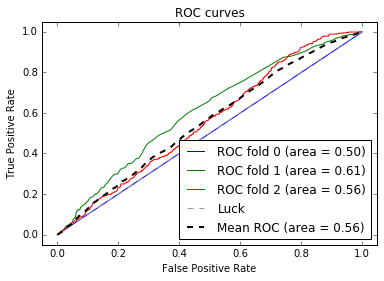
\includegraphics[width=6cm, height=5cm]{Images/svm.png}
				\label{fig:svm_roc}
				\caption{ROC curves for SVM}
			\end{figure}
		\subsection{Logistic Regression}
		\begin{figure}[H]
				\centering
				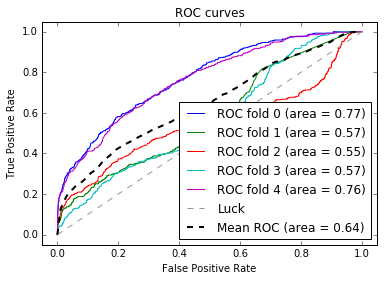
\includegraphics[width=6cm, height=5cm]{Images/logistic.png}
				\label{fig:log_roc}
				\caption{ROC curves for logistic regression}
			\end{figure}
		\subsection{Boosted Trees Classifier}
		\begin{figure}[H]
				\centering
				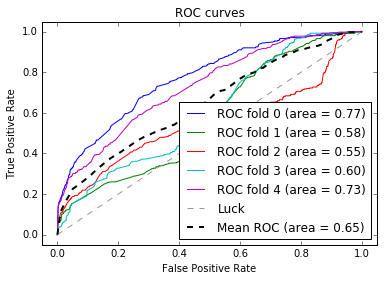
\includegraphics[width=6cm, height=5cm]{Images/boostedtrees.png}
				\label{fig:boosted_roc}
				\caption{ROC curves for boosted trees}
			\end{figure}
	\section{Results and Evaluation}
	\section{Conclusion}
	\section{Task Distribution}
\end{document}